\documentclass[12pt,a4paper]{article}

\usepackage[margin=1in]{geometry}
\usepackage[T1]{fontenc}
\usepackage[utf8]{inputenc}
\usepackage{array}
\usepackage{booktabs}
\usepackage{tabularx}
\usepackage{float}
\usepackage{graphicx}
\usepackage{xcolor}
\usepackage{listings}
\usepackage{tikz}
\usepackage{hyperref}

\usetikzlibrary{arrows.meta,backgrounds,calc,fit,positioning,shapes.geometric,shapes.symbols}

\hypersetup{
    colorlinks=true,
    linkcolor=blue!60!black,
    urlcolor=blue!60!black,
    citecolor=blue!60!black,
    pdftitle={Design and Implementation of a Multi-Service Network Using Cisco Packet Tracer},
    pdfauthor={University of Tabuk}
}

\definecolor{iosgray}{RGB}{245,245,245}
\definecolor{iosblue}{RGB}{31,78,121}
\definecolor{boxblue}{RGB}{226,239,255}
\definecolor{boxgreen}{RGB}{226,248,232}
\definecolor{boxorange}{RGB}{255,242,224}

\lstdefinelanguage{CiscoIOS}{
    sensitive=false,
    morecomment=[l]!,
    morekeywords={
        access-list,address,auto-summary,configure,description,dns-server,dot1Q,
        enable,encapsulation,eigrp,exit,FastEthernet,Ethernet,hostname,inside,
        interface,ip,list,mode,nat,network,no,outside,overload,permit,pool,
        portfast,redistribute,rip,router,shutdown,source,spanning-tree,switchport,
        terminal,trunk,vlan,version
    }
}

\lstdefinestyle{cisco}{
    language=CiscoIOS,
    backgroundcolor=\color{iosgray},
    basicstyle=\ttfamily\small,
    breaklines=true,
    columns=fullflexible,
    frame=single,
    keepspaces=true,
    keywordstyle=\color{iosblue}\bfseries,
    showstringspaces=false,
    tabsize=2,
    captionpos=b
}

\lstset{style=cisco}

\newcolumntype{Y}{>{\raggedright\arraybackslash}X}
\newcolumntype{L}[1]{>{\raggedright\arraybackslash}p{#1}}
\newcolumntype{C}[1]{>{\centering\arraybackslash}p{#1}}
\newcommand{\ip}[1]{\mbox{\texttt{#1}}}
\renewcommand{\arraystretch}{1.18}

\begin{document}

\begin{titlepage}
    \centering
    {\Large University of Tabuk\par}
    \vspace{0.15cm}
    {\large Faculty of Computers \& Information Technology\par}
    \vspace{0.15cm}
    {\large Department of Computer Engineering\par}
    \vspace{1.5cm}
    {\large CEN-431 - Computer Networks Lab\par}
    \vspace{1.7cm}
    {\Huge\bfseries Design and Implementation of a Multi-Service Network Using Cisco Packet Tracer\par}
    \vspace{1.8cm}
    {\large\textbf{Student Name}\par}
    \vspace{0.3cm}
    {\large Meshal Alanazi\par}
    \vfill
    {\large \today\par}
\end{titlepage}

\tableofcontents
\newpage

\section{Introduction}

This report presents the design and implementation of a multi-service enterprise network developed in Cisco Packet Tracer for the \textbf{CEN-431 - Computer Networks Lab} course. The project connects a main office, a core/WAN segment, and a branch office using switched VLANs, router-on-a-stick inter-VLAN routing, dynamic routing, centralized services, wireless access, and NAT/PAT Internet access.

The network was designed to separate departments into logical broadcast domains while still allowing controlled end-to-end communication through routing. The main office uses VLANs for HR, finance, IT, access, and management networks. The branch office uses separate HR-Branch and Financial VLANs and provides wireless visitor connectivity through the SSID \texttt{Branch\_Visitors}. Centralized DHCP and primary DNS services are hosted on the server farm, while the internal web server and secondary DNS service are placed in the datacenter subnet.

The main objectives of the project are:
\begin{itemize}
    \item Implement VLAN segmentation and trunking on Cisco 2960 switches.
    \item Configure inter-VLAN routing using router subinterfaces and \texttt{encapsulation dot1Q}.
    \item Use EIGRP and RIP with route redistribution between the main/core and branch routing domains.
    \item Provide DHCP, DNS, web, wireless, and NAT/PAT services.
    \item Verify connectivity across VLANs, WAN links, wireless clients, internal services, and Internet-facing paths.
\end{itemize}

\section{Network Topology \& Design}

The topology is divided into three main areas: \textbf{Main Office}, \textbf{Core/WAN}, and \textbf{Branch Office}. The core router acts as the redistribution point between EIGRP and RIP. The main office edge router provides router-on-a-stick inter-VLAN routing and NAT/PAT toward the Internet cloud. The branch router uses RIP and provides router-on-a-stick routing for VLAN 40 and VLAN 50.

\begin{figure}[H]
    \centering
    \resizebox{\textwidth}{!}{%
    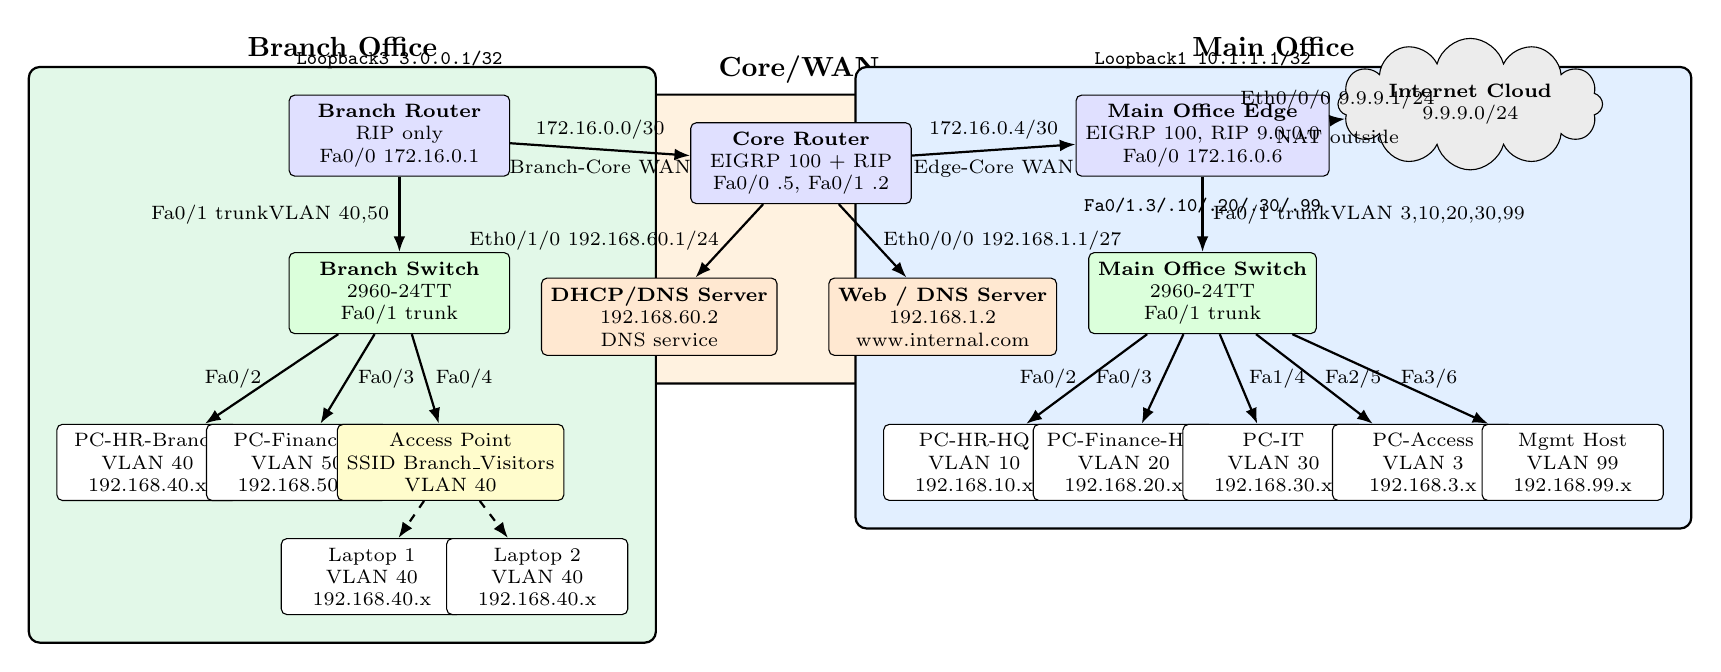
\begin{tikzpicture}[
        font=\scriptsize,
        router/.style={draw,rounded corners=2pt,fill=blue!12,minimum width=2.8cm,minimum height=0.9cm,align=center},
        switch/.style={draw,rounded corners=2pt,fill=green!14,minimum width=2.8cm,minimum height=0.8cm,align=center},
        server/.style={draw,rounded corners=2pt,fill=orange!18,minimum width=2.7cm,minimum height=0.8cm,align=center},
        pc/.style={draw,rounded corners=2pt,fill=white,minimum width=2.3cm,minimum height=0.72cm,align=center},
        ap/.style={draw,rounded corners=2pt,fill=yellow!20,minimum width=2.3cm,minimum height=0.72cm,align=center},
        netcloud/.style={draw,shape=cloud,cloud puffs=12,cloud ignores aspect,fill=gray!15,minimum width=2.5cm,minimum height=1.15cm,align=center},
        link/.style={-{Latex[length=2mm]},thick},
        wlan/.style={-{Latex[length=2mm]},thick,dashed},
        areabox/.style={draw,rounded corners=4pt,thick,inner sep=0.35cm}
    ]

        \node[router] (core) at (0,0.5) {\textbf{Core Router}\\EIGRP 100 + RIP\\Fa0/0 .5, Fa0/1 .2};
        \node[server] (dhcp) at (-1.8,-1.45) {\textbf{DHCP/DNS Server}\\192.168.60.2\\DNS service};
        \node[server] (web) at (1.8,-1.45) {\textbf{Web / DNS Server}\\192.168.1.2\\www.internal.com};

        \node[router] (edge) at (5.1,0.85) {\textbf{Main Office Edge}\\EIGRP 100, RIP 9.0.0.0\\Fa0/0 172.16.0.6};
        \node[switch] (mainsw) at (5.1,-1.15) {\textbf{Main Office Switch}\\2960-24TT\\Fa0/1 trunk};
        \node[netcloud] (internet) at (8.5,1.25) {\textbf{Internet Cloud}\\9.9.9.0/24};

        \node[pc] (pc10) at (2.2,-3.3) {PC-HR-HQ\\VLAN 10\\192.168.10.x};
        \node[pc] (pc20) at (4.1,-3.3) {PC-Finance-HQ\\VLAN 20\\192.168.20.x};
        \node[pc] (pc30) at (6.0,-3.3) {PC-IT\\VLAN 30\\192.168.30.x};
        \node[pc] (pc3) at (7.9,-3.3) {PC-Access\\VLAN 3\\192.168.3.x};
        \node[pc] (pc99) at (9.8,-3.3) {Mgmt Host\\VLAN 99\\192.168.99.x};

        \node[router] (branch) at (-5.1,0.85) {\textbf{Branch Router}\\RIP only\\Fa0/0 172.16.0.1};
        \node[switch] (branchsw) at (-5.1,-1.15) {\textbf{Branch Switch}\\2960-24TT\\Fa0/1 trunk};
        \node[pc] (pc40) at (-8.3,-3.3) {PC-HR-Branch\\VLAN 40\\192.168.40.x};
        \node[pc] (pc50) at (-6.4,-3.3) {PC-Financial\\VLAN 50\\192.168.50.x};
        \node[ap] (ap0) at (-4.45,-3.3) {Access Point\\SSID Branch\_Visitors\\VLAN 40};
        \node[pc] (lap1) at (-5.45,-4.75) {Laptop 1\\VLAN 40\\192.168.40.x};
        \node[pc] (lap2) at (-3.35,-4.75) {Laptop 2\\VLAN 40\\192.168.40.x};

        \draw[link] (branch) -- node[above] {172.16.0.0/30} node[below] {Branch-Core WAN} (core);
        \draw[link] (core) -- node[above] {172.16.0.4/30} node[below] {Edge-Core WAN} (edge);
        \draw[link] (edge) -- node[above] {Eth0/0/0 9.9.9.1/24} node[below] {NAT outside} (internet);

        \draw[link] (core) -- node[left] {Eth0/1/0 192.168.60.1/24} (dhcp);
        \draw[link] (core) -- node[right] {Eth0/0/0 192.168.1.1/27} (web);

        \draw[link] (edge) -- node[right] {Fa0/1 trunk\\VLAN 3,10,20,30,99} (mainsw);
        \draw[link] (branch) -- node[left] {Fa0/1 trunk\\VLAN 40,50} (branchsw);

        \draw[link] (mainsw) -- node[left] {Fa0/2} (pc10);
        \draw[link] (mainsw) -- node[left] {Fa0/3} (pc20);
        \draw[link] (mainsw) -- node[right] {Fa1/4} (pc30);
        \draw[link] (mainsw) -- node[right] {Fa2/5} (pc3);
        \draw[link] (mainsw) -- node[right] {Fa3/6} (pc99);

        \draw[link] (branchsw) -- node[left] {Fa0/2} (pc40);
        \draw[link] (branchsw) -- node[right] {Fa0/3} (pc50);
        \draw[link] (branchsw) -- node[right] {Fa0/4} (ap0);
        \draw[wlan] (ap0) -- (lap1);
        \draw[wlan] (ap0) -- (lap2);

        \node[below=0.15cm of edge] {\texttt{Fa0/1.3/.10/.20/.30/.99}};
        \node[above=0.2cm of edge] {\texttt{Loopback1 10.1.1.1/32}};
        \node[above=0.2cm of branch] {\texttt{Loopback3 3.0.0.1/32}};

        \begin{scope}[on background layer]
            \node[areabox,fill=boxorange,fit=(core)(dhcp)(web),label={[font=\bfseries]above:Core/WAN}] {};
            \node[areabox,fill=boxblue,fit=(edge)(mainsw)(pc10)(pc20)(pc30)(pc3)(pc99),label={[font=\bfseries]above:Main Office}] {};
            \node[areabox,fill=boxgreen,fit=(branch)(branchsw)(pc40)(pc50)(ap0)(lap1)(lap2),label={[font=\bfseries]above:Branch Office}] {};
        \end{scope}
    \end{tikzpicture}}
    \caption{Logical topology of the multi-service network using TikZ.}
    \label{fig:topology}
\end{figure}

\begin{figure}[H]
    \centering
    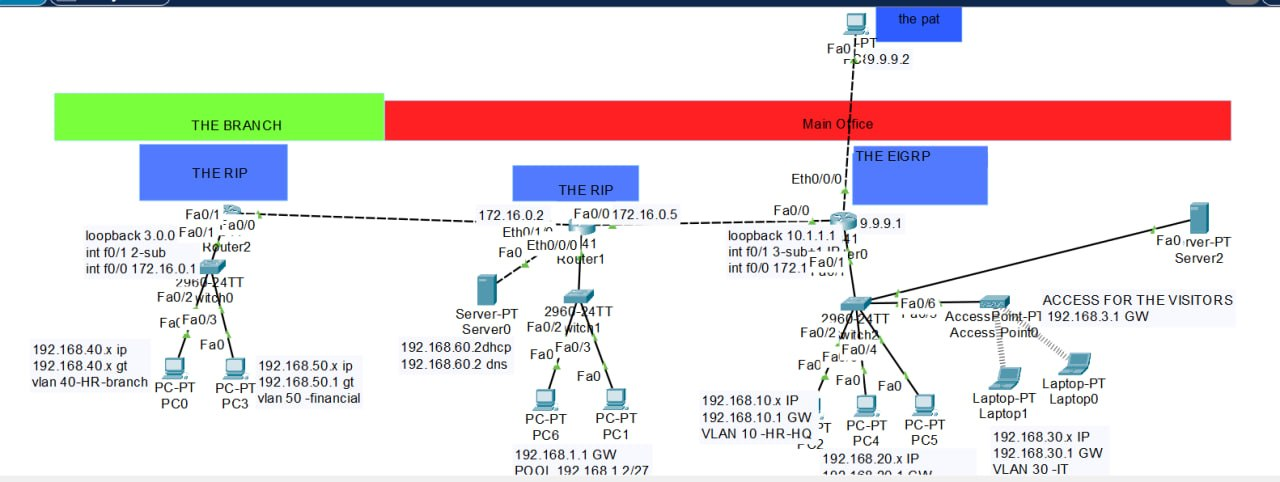
\includegraphics[width=\textwidth]{packet_tracer_topology.jpeg}
    \caption{Cisco Packet Tracer implementation screenshot of the designed network.}
    \label{fig:packet-tracer-topology}
\end{figure}

\subsection*{IP Addressing and Subnet Summary}

\begin{table}[H]
    \centering
    \footnotesize
    \caption{IP subnet and addressing summary.}
    \label{tab:subnets}
    \setlength{\tabcolsep}{3pt}
    \begin{tabularx}{\textwidth}{@{}L{3.85cm}L{2.6cm}C{1.1cm}Y@{}}
        \hline
        \textbf{Network / VLAN} & \textbf{Subnet} & \textbf{Hosts} & \textbf{Gateway / Purpose} \\
        \hline
        Internet & \ip{9.9.9.0/24} & 254 & Edge \ip{9.9.9.1}; NAT outside and Internet cloud \\
        \hline
        Branch-Core WAN & \ip{172.16.0.0/30} & 2 & Branch \ip{172.16.0.1}; Core \ip{172.16.0.2}; WAN link \\
        \hline
        Edge-Core WAN & \ip{172.16.0.4/30} & 2 & Core \ip{172.16.0.5}; Edge \ip{172.16.0.6}; WAN link \\
        \hline
        VLAN 3 (Access) & \ip{192.168.3.0/24} & 254 & Gateway \ip{192.168.3.1}; access network \\
        \hline
        VLAN 10 (HR-HQ) & \ip{192.168.10.0/24} & 254 & Gateway \ip{192.168.10.1}; main office HR \\
        \hline
        VLAN 20 (Finance-HQ) & \ip{192.168.20.0/24} & 254 & Gateway \ip{192.168.20.1}; main office finance \\
        \hline
        VLAN 30 (IT) & \ip{192.168.30.0/24} & 254 & Gateway \ip{192.168.30.1}; main office IT \\
        \hline
        VLAN 40 (HR-Branch) & \ip{192.168.40.0/24} & 254 & Gateway \ip{192.168.40.1}; branch HR and wireless clients \\
        \hline
        VLAN 50 (Financial) & \ip{192.168.50.0/24} & 254 & Gateway \ip{192.168.50.1}; branch financial users \\
        \hline
        VLAN 99 (Mgmt.) & \ip{192.168.99.0/24} & 254 & Gateway \ip{192.168.99.1}; management network \\
        \hline
        Datacenter & \ip{192.168.1.0/27} & 30 & Gateway \ip{192.168.1.1}; web and secondary DNS server \\
        \hline
        Server farm & \ip{192.168.60.0/24} & 254 & Gateway \ip{192.168.60.1}; DHCP and primary DNS server \\
        \hline
        Edge loopback & \ip{10.1.1.1/32} & 1 & Edge \texttt{Loopback1}; router identification \\
        \hline
        Branch loopback & \ip{3.0.0.1/32} & 1 & Branch \texttt{Loopback3}; router identification \\
        \hline
    \end{tabularx}
\end{table}

The usable-host values show the normal number of assignable addresses after excluding the network and broadcast addresses. The loopback addresses are /32 host routes, so each one represents a single usable host address.

\section{Switching and VLAN Configuration}

Switching was implemented using Cisco 2960-24TT switches. Instead of listing every repeated command, this report shows the important command pattern and explains how it was applied. The same access-port pattern was repeated for each user VLAN.

\subsection{Main Office Switch Configuration}

The \textbf{Main Office Switch} uses \texttt{spanning-tree mode pvst}. Interface \texttt{Fa0/1} is the trunk toward the \textbf{Main Office Edge Router}, and it carries VLANs 3, 10, 20, 30, and 99. Access ports were assigned as follows: \texttt{Fa0/2} to VLAN 10, \texttt{Fa0/3} to VLAN 20, \texttt{Fa1/4} to VLAN 30, \texttt{Fa2/5} to VLAN 3, and \texttt{Fa3/6} to VLAN 99.

\begin{lstlisting}[caption={Simplified main office switch command pattern.}]
spanning-tree mode pvst

interface FastEthernet0/1
 description Trunk_to_Edge_Router
 switchport mode trunk
 switchport trunk allowed vlan 3,10,20,30,99

interface FastEthernet0/2
 description HR-HQ
 switchport mode access
 switchport access vlan 10
 spanning-tree portfast
\end{lstlisting}

The final access-port commands were repeated for VLAN 20, VLAN 30, VLAN 3, and VLAN 99 with the correct interface number, description, and VLAN ID.

\subsection{Branch Switch Configuration}

The \textbf{Branch Switch} also uses \texttt{spanning-tree mode pvst}. Interface \texttt{Fa0/1} is the trunk toward the \textbf{Branch Router}. Interface \texttt{Fa0/2} is assigned to VLAN 40 with description \texttt{HR-BRANCH}, \texttt{Fa0/3} is assigned to VLAN 50 with description \texttt{financial}, and the wireless access point is connected as an access port in VLAN 40.

\begin{lstlisting}[caption={Simplified branch switch command pattern.}]
spanning-tree mode pvst

interface FastEthernet0/1
 description Trunk_to_Branch_Router
 switchport mode trunk
 switchport trunk allowed vlan 40,50

interface FastEthernet0/2
 description HR-BRANCH
 switchport mode access
 switchport access vlan 40
 spanning-tree portfast
\end{lstlisting}

The same access-port command pattern was used for \texttt{Fa0/3} in VLAN 50 and for the access point port in VLAN 40.

\section{Routing Protocols \& Inter-VLAN Routing}

Router-on-a-stick routing was used on the main office edge router and on the branch router. Each VLAN is represented by a router subinterface configured with \texttt{encapsulation dot1Q}. DHCP relay was enabled with \texttt{ip helper-address 192.168.60.2} so that clients in different VLANs can reach the centralized DHCP server.

Dynamic routing was divided into two routing domains. The main office and core networks use EIGRP process \texttt{100}. The branch side uses RIP. The \textbf{Core Router} performs mutual redistribution between EIGRP and RIP using explicit seed metrics to ensure redistributed routes are accepted.

\subsection{Main Office Edge Router Configuration}

The \textbf{Main Office Edge Router} connects to the core through \texttt{Fa0/0 172.16.0.6/30}, routes the main office VLANs through \texttt{Fa0/1} subinterfaces, and connects to the Internet cloud through \texttt{Eth0/0/0 9.9.9.1/24}. The following example shows the pattern used for all main office VLAN subinterfaces.

\begin{lstlisting}[caption={Simplified edge router inter-VLAN and NAT command pattern.}]
interface FastEthernet0/1.10
 description VLAN_10_HR-HQ
 encapsulation dot1Q 10
 ip address 192.168.10.1 255.255.255.0
 ip helper-address 192.168.60.2
 ip nat inside

interface Ethernet0/0/0
 description NAT_Outside_to_Internet
 ip address 9.9.9.1 255.255.255.0
 ip nat outside

access-list 1 permit 192.168.10.0 0.0.0.255
access-list 1 permit 192.168.20.0 0.0.0.255
access-list 1 permit 192.168.30.0 0.0.0.255
access-list 1 permit 192.168.40.0 0.0.0.255
access-list 1 permit 192.168.50.0 0.0.0.255
ip nat inside source list 1 interface Ethernet0/0/0 overload
\end{lstlisting}

The same subinterface pattern was repeated for VLAN 3, VLAN 20, VLAN 30, and VLAN 99. The corrected NAT ACL also included the WAN subnets \texttt{172.16.0.0/30} and \texttt{172.16.0.4/30}, plus the datacenter subnet \texttt{192.168.1.0/27}.

\subsection{Core Router Configuration}

The \textbf{Core Router} connects the main office edge router, the branch router, the datacenter subnet, and the server farm subnet. Its most important routing role is redistribution between EIGRP and RIP.

\begin{lstlisting}[caption={Simplified core router route redistribution commands.}]
router eigrp 100
 no auto-summary
 network 172.16.0.4 0.0.0.3
 network 192.168.1.0 0.0.0.31
 network 192.168.60.0 0.0.0.255
 redistribute rip metric 10000 0 255 1 1500

router rip
 version 2
 no auto-summary
 network 172.16.0.0
 redistribute eigrp 100 metric 3
\end{lstlisting}

The EIGRP redistribution metric \texttt{10000 0 255 1 1500} provides a seed metric for RIP routes entering EIGRP. The RIP redistribution metric \texttt{3} provides a hop-count seed metric for EIGRP routes entering RIP.

\subsection{Branch Router Configuration}

The \textbf{Branch Router} uses RIP and provides inter-VLAN routing for VLAN 40 and VLAN 50. VLAN 40 is used by HR-Branch users and wireless clients, while VLAN 50 is used by financial users.

\begin{lstlisting}[caption={Simplified branch router inter-VLAN and RIP commands.}]
interface FastEthernet0/1.40
 description VLAN_40_HR-BRANCH
 encapsulation dot1Q 40
 ip address 192.168.40.1 255.255.255.0
 ip helper-address 192.168.60.2

interface FastEthernet0/1.50
 description VLAN_50_financial
 encapsulation dot1Q 50
 ip address 192.168.50.1 255.255.255.0
 ip helper-address 192.168.60.2

router rip
 version 2
 no auto-summary
 network 172.16.0.0
 network 192.168.40.0
 network 192.168.50.0
\end{lstlisting}

\section{Network Services}

The project uses a centralized server model. The DHCP server and primary DNS server are located at \texttt{192.168.60.2} in the server farm subnet. A second DNS service is also configured on \texttt{192.168.1.2} in the datacenter subnet. DHCP relay is configured on router subinterfaces using \texttt{ip helper-address 192.168.60.2}, allowing clients from all VLANs to receive addresses from the correct pools.

\subsection{DHCP Server Configuration}

\begin{table}[H]
    \centering
    \footnotesize
    \caption{DHCP pools configured on the server at \texttt{192.168.60.2}.}
    \label{tab:dhcp}
    \begingroup
    \renewcommand{\arraystretch}{1.25}
    \setlength{\tabcolsep}{7pt}
    \resizebox{\textwidth}{!}{%
    \begin{tabular}{@{}lllll@{}}
        \hline
        \textbf{Pool Name} & \textbf{Network} & \textbf{Gateway} & \textbf{Hosts} & \textbf{DNS Servers} \\
        \hline
        vlan 3 access & \ip{192.168.3.0/24} & \ip{192.168.3.1} & 254 & \ip{192.168.60.2}, \ip{192.168.1.2} \\
        \hline
        datacenter & \ip{192.168.1.0/27} & \ip{192.168.1.1} & 30 & \ip{192.168.60.2}, \ip{192.168.1.2} \\
        \hline
        VLAN10 & \ip{192.168.10.0/24} & \ip{192.168.10.1} & 254 & \ip{192.168.60.2}, \ip{192.168.1.2} \\
        \hline
        VLAN20 & \ip{192.168.20.0/24} & \ip{192.168.20.1} & 254 & \ip{192.168.60.2}, \ip{192.168.1.2} \\
        \hline
        VLAN30 & \ip{192.168.30.0/24} & \ip{192.168.30.1} & 254 & \ip{192.168.60.2}, \ip{192.168.1.2} \\
        \hline
        VLAN40 & \ip{192.168.40.0/24} & \ip{192.168.40.1} & 254 & \ip{192.168.60.2}, \ip{192.168.1.2} \\
        \hline
        VLAN50 & \ip{192.168.50.0/24} & \ip{192.168.50.1} & 254 & \ip{192.168.60.2}, \ip{192.168.1.2} \\
        \hline
        serverPool & \ip{192.168.60.0/24} & \ip{0.0.0.0} & 254 & \ip{192.168.60.2}, \ip{192.168.1.2} \\
        \hline
    \end{tabular}}
    \endgroup
\end{table}

The usable-host column shows the number of normal assignable host addresses in each pool. In practice, some of these addresses may be reserved for gateways, servers, or network devices.

\subsection{DNS and Web Service}

Two DNS services were configured for name resolution. The primary DNS server is \texttt{192.168.60.2}, and the secondary DNS server is \texttt{192.168.1.2}. The required DNS A record is:

\begin{center}
    \texttt{www.internal.com} $\rightarrow$ \texttt{192.168.1.2}
\end{center}

The internal web server is placed in the datacenter subnet at \texttt{192.168.1.2}. Clients from the main office, branch office, and wireless VLAN can resolve \texttt{www.internal.com} and reach the web service after routing and DHCP relay are configured correctly.

\subsection{Wireless Service}

The wireless access point is connected to the \textbf{Branch Switch} and bridged to VLAN 40. The access point was configured with SSID \texttt{Branch\_Visitors}, WPA2-PSK using AES encryption, and channel \texttt{6}. Wireless clients receive DHCP addresses from the VLAN 40 pool and use \texttt{192.168.40.1} as their default gateway.

\section{Testing and Verification}

Testing was performed after completing VLAN, trunking, routing, DHCP, DNS, NAT/PAT, and wireless configurations. The following checks confirmed that the network operates as designed.

\begin{enumerate}
    \item \textbf{Inter-VLAN pings:} A PC in VLAN 10 successfully pinged a PC in VLAN 30. This confirmed that the main office router-on-a-stick configuration on \textbf{R-EDGE} was routing between VLAN subinterfaces correctly.

    \item \textbf{DHCP verification:} The command \texttt{ipconfig /renew} was executed on client PCs. Each client received the correct IP address, subnet mask, default gateway, and DNS server settings from its assigned pool. All VLAN clients received addresses from the correct DHCP pools hosted on \texttt{192.168.60.2}, with DNS pointing to \texttt{192.168.60.2} and \texttt{192.168.1.2}.

    \item \textbf{End-to-end routing and NAT/PAT:} A branch PC successfully pinged the main office web server at \texttt{192.168.1.2} and the Internet-facing address \texttt{9.9.9.1}. On the edge router, \texttt{show ip nat translations} confirmed that PAT was translating inside addresses through \texttt{Ethernet0/0/0}.

    \item \textbf{Routing table verification:} The command \texttt{show ip route} on the \textbf{Core Router} showed EIGRP and redistributed RIP routes. The command \texttt{show ip route} on the \textbf{Branch Router} showed RIP routes learned from the core, including routes redistributed from EIGRP.

    \item \textbf{Wireless verification:} Both laptops associated with SSID \texttt{Branch\_Visitors}, received VLAN 40 DHCP addresses, and successfully reached internal resources such as \texttt{www.internal.com} as well as external resources through the edge router.
\end{enumerate}

\section{Challenges Encountered \& Resolutions}

\begin{table}[H]
    \centering
    \footnotesize
    \caption{Implementation challenges and applied resolutions.}
    \label{tab:challenges}
    \setlength{\tabcolsep}{3pt}
    \begin{tabularx}{\textwidth}{@{}L{4.6cm}Y@{}}
        \hline
        \textbf{Challenge} & \textbf{Resolution} \\
        \hline
        ACL typos such as \texttt{192.169.x.x} prevented NAT for some internal subnets. & The NAT ACL was corrected to use the proper \texttt{192.168.x.x} networks. \\
        \hline
        DHCP broadcasts were blocked at router boundaries. & The command \texttt{ip helper-address 192.168.60.2} was added on all router subinterfaces that serve client VLANs. \\
        \hline
        Route redistribution was missing seed metrics. & Seed metrics were added on the \textbf{Core Router}: \texttt{redistribute rip metric 10000 0 255 1 1500} for EIGRP and \texttt{redistribute eigrp 100 metric 3} for RIP. \\
        \hline
        VLAN description mismatch existed on branch router subinterfaces. & Descriptions were corrected to match the switch access VLANs: \texttt{HR-BRANCH} for VLAN 40 and \texttt{financial} for VLAN 50. \\
        \hline
    \end{tabularx}
\end{table}

\section{Pros and Cons / Lessons Learned}

\subsection*{Pros}
\begin{itemize}
    \item \textbf{Scalability:} The VLAN-based structure allows new departments and access networks to be added with limited disruption.
    \item \textbf{Fast EIGRP convergence:} EIGRP improves convergence in the core and main office routing domain.
    \item \textbf{Centralized DHCP and two DNS services:} Central DHCP simplifies address management, while primary and secondary DNS improve name-resolution availability.
    \item \textbf{PAT security:} PAT hides internal client addresses when they access the Internet-facing network.
    \item \textbf{Wireless protection:} WPA2-PSK with AES provides stronger wireless access protection than open authentication.
\end{itemize}

\subsection*{Cons}
\begin{itemize}
    \item \textbf{Single point of failure:} The core router is a critical dependency for communication between the main office, branch, datacenter, and server farm.
    \item \textbf{Router-on-a-stick bottleneck:} Inter-VLAN traffic depends on router trunk links, which may become a bottleneck as traffic increases.
    \item \textbf{Manual ACL risk:} Manually written NAT ACLs are error-prone, as shown by the original \texttt{192.169.x.x} typo.
    \item \textbf{No redundancy:} The topology does not include backup routers, redundant WAN links, or failover paths.
    \item \textbf{RIP overhead:} RIP periodic updates are acceptable for a small branch but are less efficient than modern routing protocols.
\end{itemize}

\subsection*{Lessons Learned}
\begin{itemize}
    \item NAT ACLs must be verified carefully because a single subnet typo can prevent Internet access.
    \item DHCP relay using \texttt{ip helper-address} is essential when DHCP clients and servers are separated by routers.
    \item Route redistribution requires seed metrics; without them, routes may not be redistributed correctly.
    \item Documentation consistency matters because interface and VLAN description mismatches can slow troubleshooting.
\end{itemize}

\section{Conclusion}

The project successfully demonstrates the design and implementation of a multi-service network in Cisco Packet Tracer. The final topology separates departments using VLANs, connects the main office and branch through WAN links, supports centralized DHCP with two DNS services, provides web service access, enables wireless clients on VLAN 40, and allows inside networks to use PAT through the main office edge router.

The verification results confirm that inter-VLAN routing, DHCP relay, dynamic routing, route redistribution, NAT/PAT, and wireless access operate correctly. The project also highlights important operational lessons, especially the need to verify ACL syntax, configure helper addresses, define redistribution metrics, and maintain accurate documentation across router and switch interfaces.

\end{document}
